\documentclass{article}
\usepackage[spanish]{babel}
\usepackage{fancyhdr}
\usepackage{graphicx}
\usepackage{setspace}
\usepackage[table]{xcolor}
\usepackage{tabularx}
\usepackage{array}
\usepackage{multicol}
\usepackage{multirow}
\usepackage[margin=2.5cm]{geometry}
\usepackage{float}
\usepackage{color, colortbl}
\definecolor{tablebackground}{rgb}{0.8, 0, 0}


\newcolumntype{M}[1]{>{\centering\arraybackslash}m{#1}}
\newcolumntype{N}{>{\centering\arraybackslash}p{3.5cm}}
\newcolumntype{x}[1]{>{\centering\arraybackslash}p{#1}}

\pagestyle{fancy}
\lhead{\begin{picture}(0,0) \put(0,0){
\includegraphics[width=30mm]{img/logoSistemas.png}} \end{picture}}
\rhead{\begin{picture}(0,0) \put(-33,5){
\includegraphics[width=12mm]{./img/logoAbet.png}} \end{picture}}
\renewcommand{\headrulewidth}{0.5pt}

\fancyhead[C]{
 	\tiny Universidad Nacional de San Agustín de Arequipa \\
  	Facultad de Ingeniería de Producción y Servicios \\
  	Departamento de Ingeniería de Sistemas e Informática \\
  	Escuela Profesional de Ingeniería de Sistemas \\
  	\textbf{Programación Web 2}
}

\fancyfoot[L]{Estudiante Rafael Nina Calizaya}
\fancyfoot[C]{Pag. \thepage}
\fancyfoot[R]{Programación Web 2}
\renewcommand{\footrulewidth}{0.5pt}


\newcommand{\itemNombre}{Rafael Diego Nina Calizaya}
\newcommand{\itemCorreo}{rninacal@unsa.edu.pe}
\newcommand{\itemEscuela}{Escuela Profesional de Ingeniería de Sistemas}
\newcommand{\itemCurso}{Programación Web 2}
\newcommand{\itemSemestre}{III}
\newcommand{\itemCodigo}{1702122}
\newcommand{\itemLaboratorio}{05}
\newcommand{\itemTema}{Python}
\newcommand{\itemSemestreAcademico}{2024-A}
\newcommand{\itemInicio}{27 Mayo 2024}
\newcommand{\itemFinal}{31 Mayo 2024}

\begin{document}
.

\begin{center}	
	\fontsize{17}{17} \textbf{ Informe de Laboratorio \itemLaboratorio}
\end{center}
\centerline{\textbf{\Large Tema: Python}}

\begin{flushright}
	\begin{tabular}{|M{2.5cm}|N|}
		\hline
		\rowcolor{tablebackground}
		\color{white} \textbf{Nota}  \\
		\hline 
		     \\[18pt]
		\hline 			
	\end{tabular}
\end{flushright}	
\begin{table}[h]
	\renewcommand{\arraystretch}{0.5}
	\hspace{2px}
	\begin{tabular}{|x{4.8cm}|x{4.8cm}|x{4.8cm}|}
		\hline 
		\rowcolor{tablebackground}
		\color{white} \textbf{Estudiante} & \color{white}\textbf{Escuela}  & \color{white}\textbf{Asignatura}   \\
		\hline 
		{\itemNombre \par \itemCorreo} & \itemEscuela & {\itemCurso \par Semestre: \itemSemestre \par Código: \itemCodigo}     \\
		\hline 			
	\end{tabular}
\end{table}		
	
\begin{table}[h]
	\renewcommand{\arraystretch}{0.5}
	\hspace{2px}
	\begin{tabular}{|x{4.8cm}|x{4.8cm}|x{4.8cm}|}
		\hline 
		\rowcolor{tablebackground}
		\color{white}\textbf{Laboratorio} & \color{white}\textbf{Tema}  & \color{white}\textbf{Duración}   \\
		\hline 
		\itemLaboratorio & \itemTema & 06  \\
		\hline 
	\end{tabular}
\end{table}

\begin{table}[h]
	\renewcommand{\arraystretch}{0.5}
	\hspace{2px}
	\begin{tabular}{|x{4.8cm}|x{4.8cm}|x{4.8cm}|}
		\hline 
		\rowcolor{tablebackground}
		\color{white}\textbf{Semestre académico} & \color{white}\textbf{Fecha de inicio}  & \color{white}\textbf{Fecha de entrega}   \\
		\hline 
		\itemSemestreAcademico & \itemInicio &  \itemFinal  \\
		\hline 
	\end{tabular}
\end{table}

\section{URL del Repositorio:}
https://github.com/DrN25/pw2\_24a/tree/main/Lab05
	
\section{Tarea:}
En esta tarea usted pondrá en práctica sus conocimientos de programación en Python para dibujar un tablero de Ajedrez.
\subsection*{Implementación de los métodos de la clase Picture.}
Se implementaron los métodos de Picture, con los procedimientos y métodos pedidos en la practica.
\begin{itemize}
    \item \textbf{verticalMirror(): } Este método retorna una copia vertical de un Picture. Ya viene implementado previamente desde el repositorio de la práctica.\\



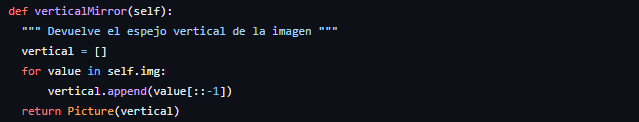
\includegraphics[width=\textwidth]{img/1.png}
\item \textbf{horizontalMirror(): } Este método retorna una copia horizontal de un Picture. Aquí solo se invierte el orden del arreglo para voltear la imagen.\\



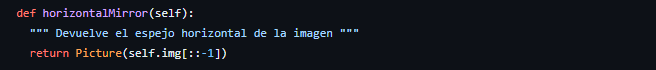
\includegraphics[width=\textwidth]{img/2.png}
\item \textbf{negative(): } Este método retorna un Picture con sus colores opuestos. Aquí se crea un arreglo de valores opuestos llamado \textbf{inverter}, obteniendo los de la clase \textbf{Color}, para luego iterar sobre cada fila y columna de la imagen, donde se invertirá los caracteres según el arreglo \textbf{inverter}, y en caso de que sea “ “ se mantendrá igual.\\



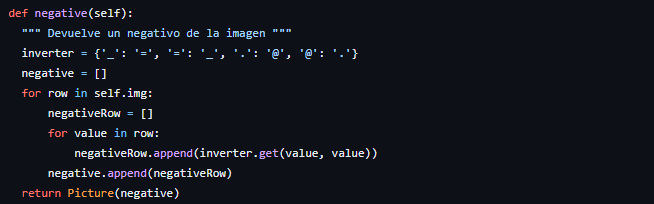
\includegraphics[width=\textwidth]{img/3.png}
\item \textbf{join(): } Este método retorna un nuevo Picture, donde Picture p está al lado derecho del Picture actual. Para conseguir ello, se itera sobre cada fila de Picture, donde en el nuevo arreglo se irán agregando cada fila del Picture actual más cada fila del Picture p.\\



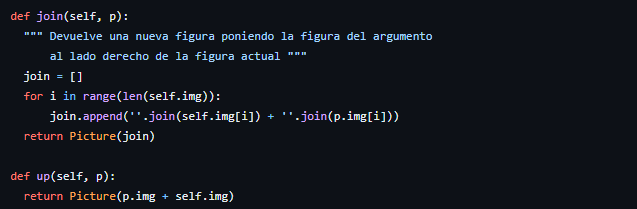
\includegraphics[width=\textwidth]{img/4.png}
\item \textbf{up(): } Este método retorna un nuevo Picture, donde el Picture actual está arriba de Picture p. Aquí solo se suman los arreglos para conseguir ello.\\



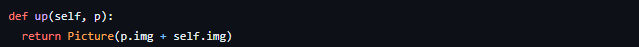
\includegraphics[width=\textwidth]{img/5.png}
\item \textbf{under(): } Este método retorna un Picture, donde Picture p se sobrepone en el Picture actual. Aquí se itera sobre cada fila y columna de los arreglos, donde cada carácter de Picture p se colocara en el nuevo arreglo, a excepción de que el carácter sea igual a " ", donde se pondrá el carácter del Picture actual correspondiente a la fila y columna de ese momento.\\



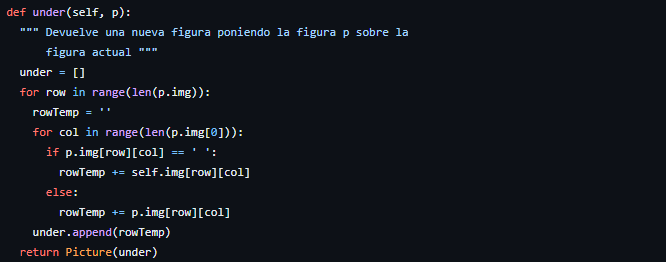
\includegraphics[width=\textwidth]{img/6.png}
\item \textbf{horizontalRepeat(): } Este método retorna un Picture que se repite n veces de manera horizontal. Para ello se itera sobre cada índice del arreglo actual, y se multiplica cada fila por la cantidad n entregada para dar como resultado las repeticiones horizontales.\\



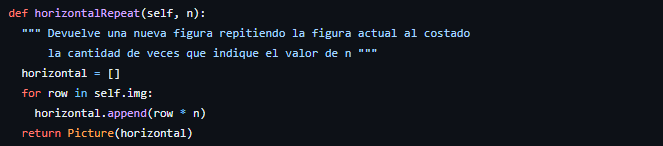
\includegraphics[width=\textwidth]{img/7.png}
\item \textbf{verticalRepeat(): } Este método retorna un Picture que se repite n veces de manera vertical. Para ello, se trabaja con un ciclo for, donde en cada ciclo se agregara la imagen actual al nuevo arreglo, y esto se repetirá n veces para dar como resultado las repeticiones verticales.\\

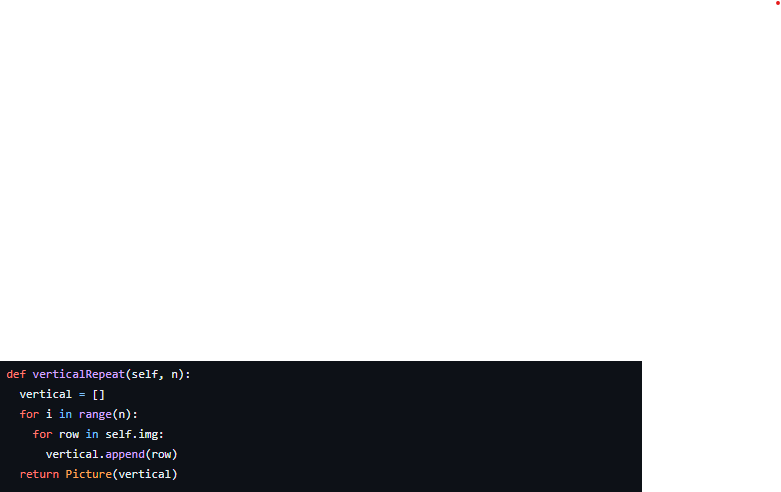
\includegraphics[width=\textwidth]{img/8.png}
\item \textbf{EXTRA: rotate(): } Esta función retorna el Picture actual rotado 90° a la derecha. Aquí mediante 2 ciclos for se itero sobre la imagen actual. utilizando la función \textbf{reversed()} para iterar sobre las filas de abajo hacia arriba, pudiendo construir la imagen rotada 90°.\\

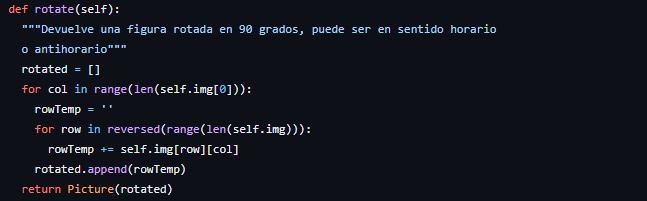
\includegraphics[width=\textwidth]{img/extra.png}
\end{itemize}

\subsection*{Ejercicios Resueltos.}

\begin{itemize}
\item \textbf{EJERCICIO A:} Se hizo uso de los métodos negative(), join() y up() para unir los caballos y cambiarlos de color.\\




\includegraphics[width=\textwidth]{img/9.png}


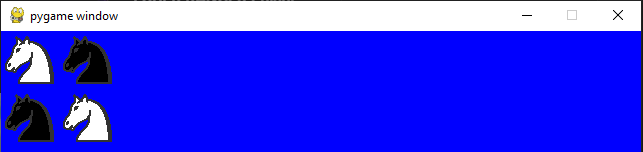
\includegraphics[width=\textwidth]{img/10.png}
\item \textbf{EJERCICIO B:} Se hizo uso de lo trabajado en el ejercicio 1 y se usó el método verticalMirror().\\



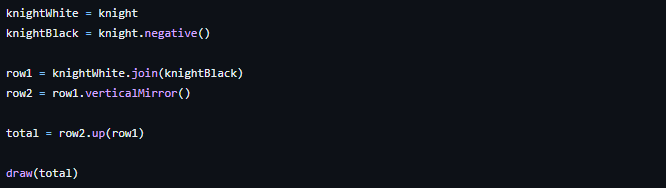
\includegraphics[width=\textwidth]{img/11.png}



\includegraphics[width=\textwidth]{img/12.png}
\item \textbf{EJERCICIO C:} Se hizo uso del método horizontalRepeat() para crear 4 reinas una al lado de la otra. \\



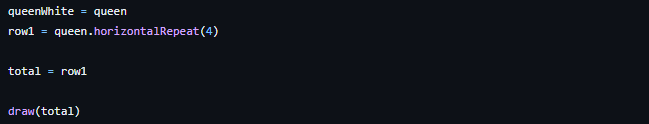
\includegraphics[width=\textwidth]{img/13.png}


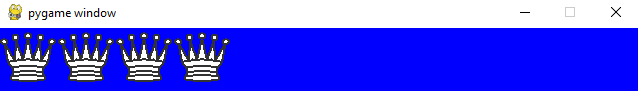
\includegraphics[width=\textwidth]{img/14.png}
\item \textbf{EJERCICIO D:} Se hizo uso de los métodos negative(), join() y horizontalRepeat(), buscando reutilizar el objeto Picture creado al inicio y no crear innecesariamente otros varios más.\\



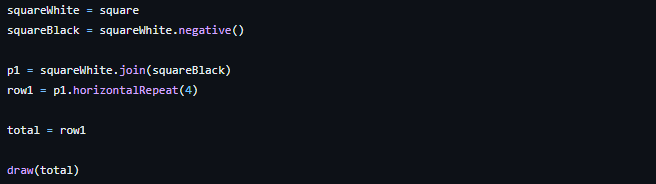
\includegraphics[width=\textwidth]{img/15.png}


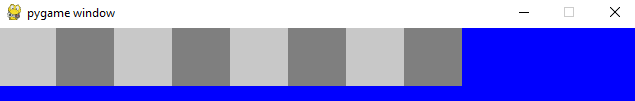
\includegraphics[width=\textwidth]{img/16.png}
\item \textbf{EJERCICIO E:} Se utilizó la solución del ejercicio 4 pero se le agrego el método negative() para obtener el resultado buscado.\\


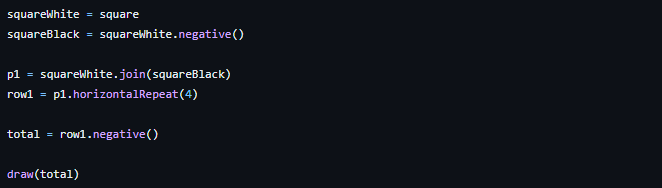
\includegraphics[width=\textwidth]{img/17.png}


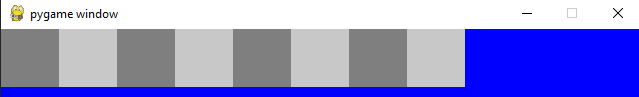
\includegraphics[width=\textwidth]{img/18.png}
\item \textbf{EJERCICIO F:} Se reutilizo la implementación de los ejercicios 4 y 5, ademas se utilizo los métodos up() y verticalRepeat().\\



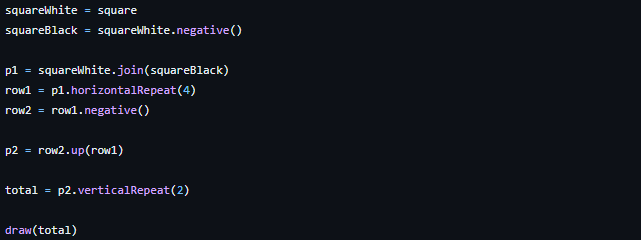
\includegraphics[width=\textwidth]{img/19.png}


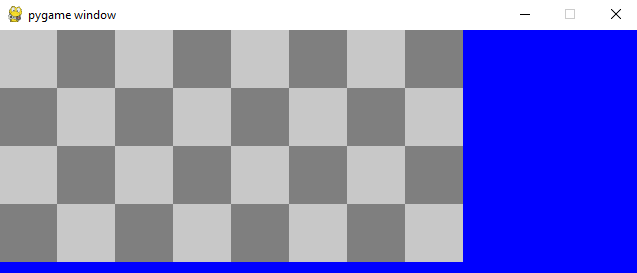
\includegraphics[width=\textwidth]{img/20.png}
\item \textbf{EJERCICIO G:} Se dividió el tablero en pequeñas subpartes las cuales se pudieran repetir o fueran el inverso de otras, por lo que se busco crear estas subpartes para al final unirlas y acomodarlas con los métodos join(), negative(), up(), verticalRepeat(), horizontalRepeat() y under(). Con esto se logró completar el tablero de ajedrez.\\



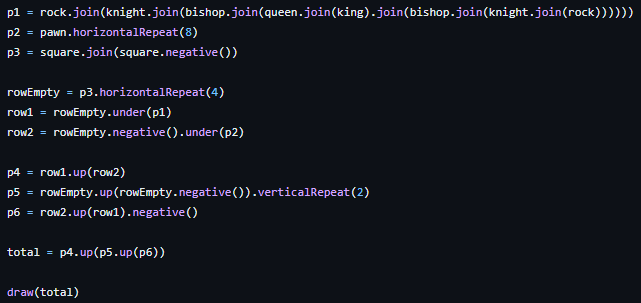
\includegraphics[width=\textwidth]{img/21.png}


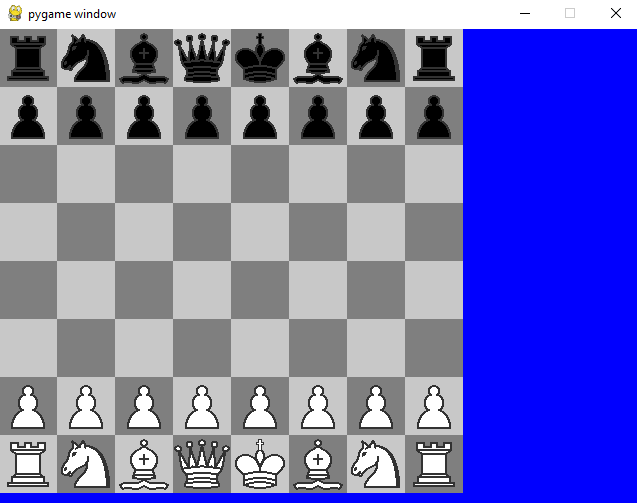
\includegraphics[width=\textwidth]{img/22.png}
\end{itemize}
\subsection*{Pregunta:}
\textbf{Explique: ¿Para qué sirve el directorio pycache?}\\
Este directorio sirve para almacenar archivos caché de byte-code generados por Python. Gracias a ello se puede optimizar en el tiempo de carga de los módulos al evitar la recompilación del código fuente cada vez que se importa un archivo .py, mejorando el rendimiento y velocidad de ejecución de los programas en Python, siendo de utilidad para proyectos a gran escala con muchos módulos de por medio.

\section{Commits realizados:}

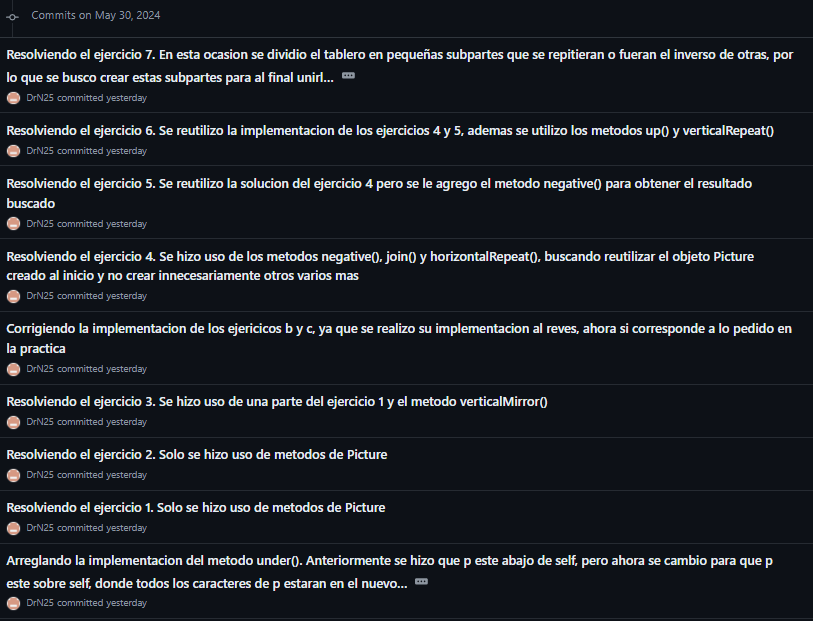
\includegraphics[width=\textwidth]{img/commits1.png}


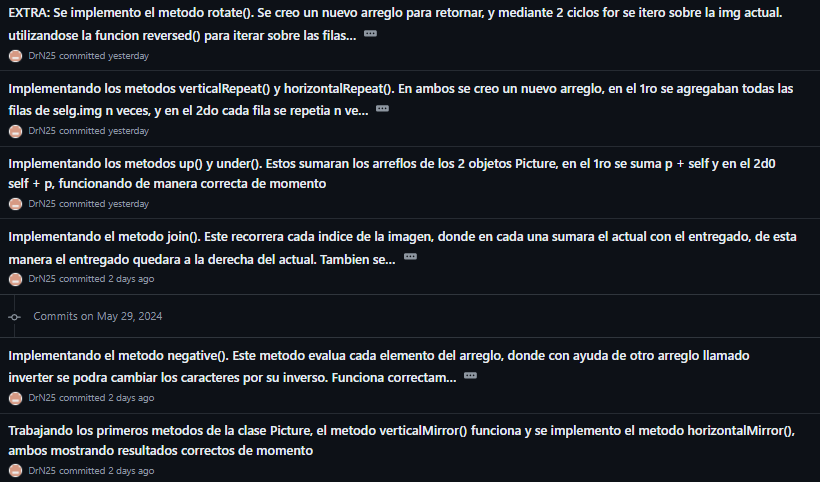
\includegraphics[width=\textwidth]{img/commits2.png}
\section{Rúbrica:}




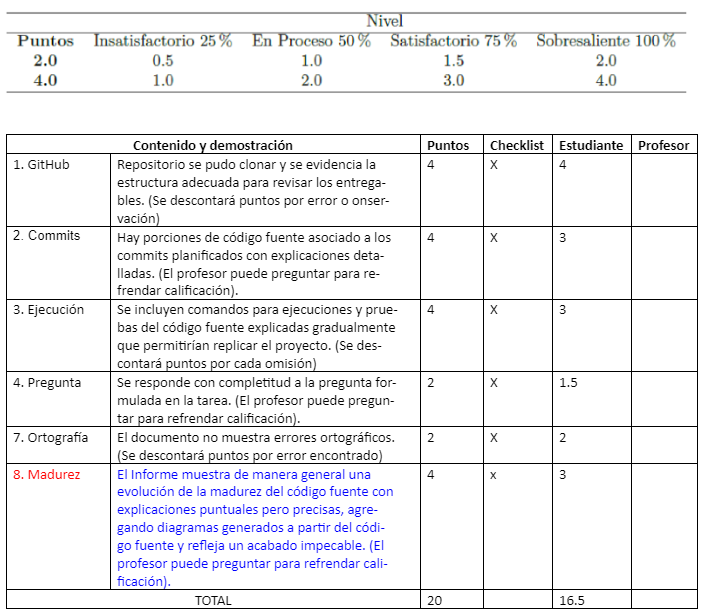
\includegraphics[width=\textwidth]{img/rubrica.png}
\end{document}